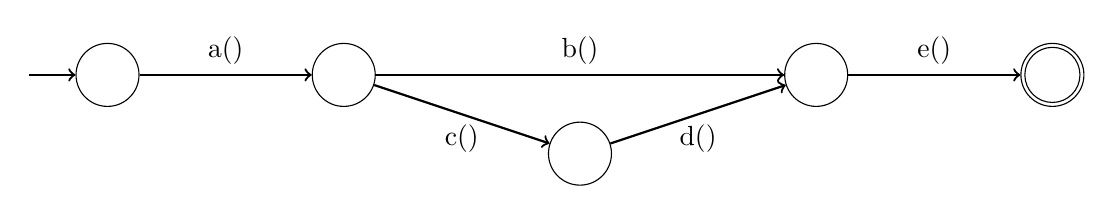
\begin{tikzpicture}[
    mystyle/.style={circle, minimum size=8mm, fill=white, draw=black}
]
    \node[mystyle] at (0,0) (n1) {};
    \node[mystyle] at (3,0) (n2) {};
    \node[mystyle] at (6,-1) (n3) {};
    \node[mystyle] at (9,0) (n4) {};
    \node[mystyle] at (12,0) (n5) {};

    \draw[->, thick] (-1,0) -- (n1);
    \draw[->, thick] (n1) -- node[above] {a()} (n2);
    \draw[->, thick] (n2) -- node[above] {b()} (n4);
    \draw[->, thick] (n4) -- node[above] {e()} (n5);
    \draw[->, thick] (n2) -- node[below] {c()} (n3);
    \draw[->, thick] (n3) -- node[below] {d()} (n4);
    \draw[] (n5) circle (3.5mm);
\end{tikzpicture}
